%%%%%%%%%%%%%%%%%%%%%%%%%%% asme2ej.tex %%%%%%%%%%%%%%%%%%%%%%%%%%%%%%%
% Template for producing ASME-format journal articles using LaTeX    %
% Written by   Harry H. Cheng, Professor and Director                %
%              Integration Engineering Laboratory                    %
%              Department of Mechanical and Aeronautical Engineering %
%              University of California                              %
%              Davis, CA 95616                                       %
%              Tel: (530) 752-5020 (office)                          %
%                   (530) 752-1028 (lab)                             %
%              Fax: (530) 752-4158                                   %
%              Email: hhcheng@ucdavis.edu                            %
%              WWW:   http://iel.ucdavis.edu/people/cheng.html       %
%              May 7, 1994                                           %
% Modified: February 16, 2001 by Harry H. Cheng                      %
% Modified: January  01, 2003 by Geoffrey R. Shiflett                %
% Use at your own risk, send complaints to /dev/null                 %
%%%%%%%%%%%%%%%%%%%%%%%%%%%%%%%%%%%%%%%%%%%%%%%%%%%%%%%%%%%%%%%%%%%%%%

%%% use twocolumn and 10pt options with the asme2ej format
\documentclass[twocolumn,10pt]{asme2ej}


\usepackage{amsthm}
\usepackage{amsmath}
% \usepackage{epsfig} %% for loading postscript figures
\usepackage{algorithm}
\usepackage{algorithmic}
\usepackage{pgfplots}
\pgfplotsset{width=7cm,compat=1.8}
\usepackage{graphicx}
\graphicspath{ {./figure/} }

\newtheorem{theorem}{Theorem}[section]
\newtheorem{lemma}[theorem]{Lemma}
\newtheorem{axiom}[theorem]{Axiom}

%% The class has several options
%  onecolumn/twocolumn - format for one or two columns per page
%  10pt/11pt/12pt - use 10, 11, or 12 point font
%  oneside/twoside - format for oneside/twosided printing
%  final/draft - format for final/draft copy
%  cleanfoot - take out copyright info in footer leave page number
%  cleanhead - take out the conference banner on the title page
%  titlepage/notitlepage - put in titlepage or leave out titlepage
%  
%% The default is oneside, onecolumn, 10pt, final


\title{Information Theory Approach to Reducing Failure Inducing Input}

%%% first author
\author{Mike Fairhurst
    \affiliation{
	Google Inc.,
    Email: mfairhurst@google.com
    }	
}

%%% second author
%%% remove the following entry for single author papers
%%% add more entries for additional authors
%%%\author{J. Michael McCarthy\thanks{Address all correspondence related to ASME style format and figures to this author.} \\
%%%    \affiliation{ Editor, Fellow of ASME\\
%%%	Journal of Mechanical Design\\
%%%        Email: jmmccart@uci.edu
%%%    }
%%%}
%%%
%%%%%% third author
%%%%%% remove the following entry for single author papers
%%%%%% add more entries for additional authors
%%%\author{Third Co-author\\
%%%        Graduate Research Assistan, Student Member of ASME\\
%%%       {\tensfb Fourth Co-author}\thanks{Address all correspondence for other issues to this author.} 
%%%    \affiliation{Title, Member of ASME\\
%%%        Department or Division Name\\
%%%        Company or College Name\\
%%%        City, State (spelled out), Zip Code\\
%%%        Country (only if not U.S.)\\
%%%        Email address (if available)
%%%    }
%%%}


\begin{document}

\maketitle    

%%%%%%%%%%%%%%%%%%%%%%%%%%%%%%%%%%%%%%%%%%%%%%%%%%%%%%%%%%%%%%%%%%%%%%
\begin{abstract}
{\it
Debugging software is easier with examples of minimal inputs that reproduce
defects. This paper introduces "entropy debugging'" an improved algorithm to
simplify failure inducing inputs that outperforms its predecessor "delta
debugging". By taking a statistical approach to a generalizable set minimization
problem, we are able to treat the pass/fail results of fitness tests as a stream
of binary information. Entropy debugging leverages data compression techniques
to minimize this stream, meaning fewer fitness tests are performed and the
algorithm approaches the upper bound of possible performance in both high
entropy (already well minimized) and low entropy (not well minimized) cases.
\end{abstract}

%%%%%%%%%%%%%%%%%%%%%%%%%%%%%%%%%%%%%%%%%%%%%%%%%%%%%%%%%%%%%%%%%%%%%%
%%%\begin{nomenclature}
%%%\entry{A}{You may include nomenclature here.}
%%%\entry{$\alpha$}{There are two arguments for each entry of the nomemclature environment, the symbol and the definition.}
%%%\end{nomenclature}
%%%
%%%The primary text heading is  boldface and flushed left with the left margin.  The spacing between the  text and the heading is two line spaces.
%%%
%%%%%%%%%%%%%%%%%%%%%%%%%%%%%%%%%%%%%%%%%%%%%%%%%%%%%%%%%%%%%%%%%%%%%%%%%
\section{Introduction}

Known reproductions of software defects often facilitate efficient debugging of
that software, however, reproductions often contain extraneous input,
complicating the troubleshooting process. Fuzz testing, a technique where
randomized inputs are fed to a program in search of unwanted behavior such as
crashes, is particularly known to produce overly complex defect-inducing inputs.
Therefore, it is sensible to employing algorithms capable of minimizing these.
Additionally, these algorthms can be valuable for for simplifying reproductions
discovered by developers or end-users.

One approach to simplifying failure-inpucing input is employing a simple
iterative algorithm which removes one character of that input at a time. For
each character that is removed, the algorithm checks that the program still
exhibits the defect of interest with the simpler input, and in this case the
extraneous character is removed.

Due to the complexity of real world programs, the removal
of one character at the end of the input may affect the necessity of a character
at the beginning. Consider a parser that crashes with unclosed parentheses given
the input string: '(((()))'. None of the open parenthesis may be removed from
the input without suppressing the crash until all closing parentheses are first
removed. To produce higher qualitity minimizations, which we refer to as
1-minimal (no single character may be removed from the reproduction without
compromising it), the simple iterative algorithm can be iterated to a fixed
point. This concept of n-minimality is defined by Zeller\cite{dd}.

% TODO: improve academic tone of "it is also worth noting"
Reaching 1-minimality in this way requires $O(n^2)$ steps where $n$ is the size,
of the failure-inducing input, and each step requires running the defective
program, which may be computationally expensive. It is also worth noting that
in real world use cases, extraneous input is also often clustered and
may constitute the majority of the reproduction. A strategy that only removes
one character at a time cannot exploit these patterns to achieve improved
efficiency in real-world scenarios.

Delta Debugging is an algorithm by Zeller\cite{dd} which can offer improved
real-world performance by removing one or more characters per test against a
target program. Delta Debugging resembles a binary
search where at the nth stage, 1/nth of the failure-inducing input is deleted
and checked against the target program. Eventually, one nth of the
failure-inducing input will be a single character. At this
point the behavior of the Delta Debugging algorithm matches the naive iterative
algorithm so that a 1-minimal reproduction may be found.

The bisection approach taken by Delta Debugging has the potential to
greatly reduce a reproduction in few tests when the failure-inducing input
contains large volumes of extraneous content. However, if a failure-inducing
input is already close to minimal, the algorithm typically
does not produce working reproductions when removing multiple characters. In
cases where the algorithm is simplifying reproduction which are already close to
1-minimal, Delta Debugging effectively functions as a slower version of the
single character iteration algorithm. This inconsistency in potential performance
is consistent with the finding by Yu et. al that the usefulness of Delta
Debugging can vary wildly in real world scenarios\cite{ddRealPerspectives}.
% TODO: read Yu et al for more info and a better sentence here.

Hierarchical Delta Debugging\cite{hdd} is a proposed variation that may improve the
effectiveness of these early steps in the Delta Debugging algorithm for certain
target programs. HDD may be employed when the target program operates on
tree-like data such as parsers and certain data decoders. A developer may create
a module which produces an abstract syntax tree (AST) from a failure-inducing
input. HDD then operates by removing branches of this tree, which is an
effective approach to quickly reduce failure-inducing inputs in certain cases.
This technique does require additional effort by the developer, and is less
suitable for many programs such as image decoders. It also may be less useful
to fuzz testers who wish to produce and simplify malformed inputs. Lastly, Yu
et. al found that Hierarchical Delta Debugging did not yield definite
improvements over Delta Debugging in efficiency in real world
application\cite{ddRealPerspectives}.

Modern "Grey Box" fuzz testing software presents a scenario that necessitates a
simplification algorithm that efficiently reduces both noisy and highly reduced
data samples.  Grey Box fuzz testing is a widely utilized and highly efficient
technique to automate the discovery of defects in software. Grey box fuzz
testing frameworks execute a target piece of software with code coverage
collection enabled. This method is also known as "code coverage guided fuzz
testing." This method involves maintaining a corpus of inputs which execute
different code paths inside the target program. This corpus is then mangled and
spliced to produce new candidate inputs, which are added to the corpus if the
corresponding execution involves new branches in the target program. For
example, if the target program is a compiler, one sample may hold a class

these two samples eventually yields a method definition, which is added to the
corpus. A minimized corpus is more likely to yield novel new samples during the
random splicing process. Extraneous data, such as lengthy comments in the case
of fuzz testing compilers, reduce the likelihood that splicing involves data of
interest (e.g. the class and function definitions). Grey Box fuzz testing
software may then wish to employ an algorithm which is capable of efficiently
simplifying all samples before adding them to the corpus, where these
unminimized samples range from nearly being 1-minimal, to containing large
sections of extraneous input.

In this paper we present "Entropy Debugging," a new algorithm which demonstrates
superior performance as compared to Delta Debugging in various scenarios.
Through an information theory based approach, our algorithm achieves more
efficient most of Zeller's original data examples\cite{dd} in significantly
fewer tests. Moreover, our algorithm demonstrates near optimal performance on
inputs which are already near 1-minimal. To support our claims we include
quantitative results on generated data as well as Zeller's test cases. Based on
these findings, we argue our algorithm represents a compelling choice for
reducing failure-inducing inputs in various scenarios, and anticipate its
effectiveness in other related areas as well.

%% \subsection{Formalizations}
%% 
%% Delta Debugging\cite{dd} and the algorithm presented here are both algorithms
%% that solve the following general problem.
%% 
%% \subsubsection{Set Minimization}
%% We define the problem of \textbf{set minimization} as $sm(\alpha, t) = \alpha'$,
%% where $\alpha$ is an ordered or unordered set, $t$ is a blackbox function, and
%% $\alpha'$ is the smallest set $s$ such that $s \subset \alpha$ and $t(s)$.
%% (Zeller's "local minimum"\cite{dd}).
%% 
%% Given that $t$ is an abritrary black box function, its performance is unbounded.
%% Therefore an important measure of complexity of an algorithm performing set
%% minimization is the number of invocations of $t$.
%% 
%% Set minimization is the true goal of both Delta Debugging and the algorithm
%% presented in this paper, however, the complexity of $sm(\alpha, t)$ is
%% $2^{|\alpha|}$\cite{dd}.
%% 
%% Therefore a different definition is needed for practical purposes; for this
%% there is \textbf{n-minimality}\cite{dd}.
%% 
%% \subsubsection{1-minimality}
%% 
%% Zeller defines \textbf{n-minimality} as $min(\alpha, t, n) = \alpha'$ where
%% $\forall c \subset \alpha \cdot |c| - |\alpha| \leq n \Rightarrow t(c)$.
%% Zeller proposes that 1-minimality is the ideal target for an algorithm
%% approximating set minimization.
%% 
%% In less formal terms, n-minimality can be defined as searching for a result
%% where no n items in the set could be removed while still satisfying the test
%% function. In the case of 1-minimal, this means that no individual item in
%% the set can be removed on its own while satisfying $t$, though it is possible
%% that some pair of entries in the set (or tuples of size $n > 1$) could be.
%% 
%% This paper disputes the value of 1-minimality, though the algorithm presented
%% can help efficiently find 1-minimal results.
%% 
%% To do: link to disputing the value of 1-minimality
%% 
%% Finding a 1-minimal set is $O(n^2)$.
%% 
%% \subsubsection{Set Simplification}
%% 
%% There is also a new presented definition, which is core to the ideas presented
%% in this paper. We define the problem of \textbf{set simplification} as
%% $simplify(\alpha, t) = \alpha'$ as a subproblem of set minimization. In
%% simplification, it is required that $t$ satisfies
%% $\forall c \supset \alpha' \Rightarrow t(c)$.
%% 
%% \begin{theorem}
%%   The worst case complexity of set simplification is $O(n)$.
%% \end{theorem}
%% 
%% \begin{axiom}
%%   $t(\alpha' \setminus {c})$ iff $c \in \alpha'$.
%% \end{axiom}
%% 
%% \begin{axiom}
%%   $|\alpha'| \leq |\alpha|$.
%% \end{axiom}
%% 
%% \begin{lemma}
%%   $simplify(\alpha, t) = \{ c | c \in \alpha, t(\alpha \setminus {c}) \}$
%% \end{lemma}
%% 
%% %%% TODO: show that it takes *at least |alpha'| steps.
%% 
%% \begin{proof}
%%   Since set simplification can be translated to a list comprehension on
%%   $\alpha$, it cannot take more than $|\alpha|$ steps to find.
%% \end{proof}
%% 
%% \begin{theorem}
%%   The result of set simplification is also n-minimal for all n.
%% \end{theorem}
%% 
%% \begin{proof}
%%   Assume that $\alpha'$ is not n-minimal for some $n > 0$. That means
%%   $\exists c \subset \alpha' \cdot |c| - |\alpha'| > n \land t(c)$. That
%%   implies $|c| < |\alpha'|$. However, if $t(c)$ and $|c| < |\alpha'|$, then
%%   $|\alpha'|$ is not the smallest $s$ such that $t(s)$. This is a contradiction.
%%   Therefore if the set simplification result $\alpha'$ is n-minimal for all n.
%% \end{proof}
%% 
%% In practice, few nontrivial tests satisfy the requirements to make set
%% simplification applicable. However, this paper uses set simplification as a
%% benchmark of algorithmic performance and suggests it as a good approximation for
%% many use cases where set minimization is desired.

%% \subsection{Information Theory Approach}
%% 
%% The novel approach taken to find a better algorithm of approximating set
%% minimization is to translate test function results into an information stream.
%% This paper explores how that information stream can be compressed efficiently.
%% 
%% Expressing the problem as a data stream is easier from the lens of \textit{set
%% simplification} than \textit{set minimization}. (Later,
%% \textit{set minimization} will be compared to noisy data streams).
%% 
%% To do: eventually compare set minimization to noisy data streams.
%% 
%% From here on, this paper assumes that $\alpha$ is a \textit{totally ordered set}.

\section{Improved Algorithm Design: A Data Compression Approach}

To construct an algorithm with improved efficiency, we apply optimistic
assumptions that simplify the problem of reducing a failure-inducing input. By
applying proper design considerations, these assumptions make it possible to
produce data compression mappings which may be reinterpreted as test invocations
in search of a 1-minimal failure inducing input. Our algorithm demonstrates high
real-world performance even when these optimistic assumptions do not hold, as
evidenced by quantatative data analysis conducted in this study. The following
section provides a detailed overview of our information-theory based approach.

For this section we introduce the concept of a minimal ordered set $\alpha$. We
define $\alpha$ to be the smallest possible ordered set which satisfies
condition $f(\alpha') = true$ for some function $f$. To facilitate algorithm
design, we assume that any superset $\alpha'$ of the minimal set $\alpha$ also
satisfies the condition $f(\alpha') = true$. These definitions and assumptions
form a foundation for our proposed problem of set simplification. In this
problem, $\alpha'$ is a known non-minimal reproduction of a defect, and $f(i)$
is true when the program of interest crashes in the relevant manner given input
$i$. The objective of our algorithm is to find the minimal reproduction,
represented by $\alpha$, in minimal invocations of function $f$.

\subsection{Simplification Stream Forms and Performance Lower Bounds}

Simplifying a non-minimal set $\alpha'$ involves identifying the important and
unimportant members within $\alpha'$. In order to leverage data compression
techniques in the search for the minimal set $\alpha$ it is necessary to
translate $\alpha$ into a binary stream.

We introduce the concept of \textit{simplification stream form}, which
represents each member $e$ in $\alpha'$ as "$i$" if $e \in \alpha$ and "$u$" if
$e \notin \alpha$. For example, a non-minimal set $\alpha'$ which contains three
"important" members is expressed as $iii$ in simplification stream form. Three
unimportant members is expressed as $uuu$. A pair of important members followed
by a pair of unimportant members is represented as $iiuu$. This form enables the
application of information theory techniques to the problem of simplifying
failure-inducing input.

The problem of minimizing a non-minimal failure-inducing input $\alpha'$ can
therefore be expressed as a search for $ssf(\alpha')$ in as few invocations of
test function $f$ as possible. The simplification stream form encapsulates all
the essential information required to derive the minimized input $\alpha$ from
$\alpha'$ without additional invocations of $f$.

Simplification stream forms also make clear an upper bound on the maximum steps
required by a simplification algorithm. The simplification stream form of any
input can always be derived in $|\alpha'|$ steps, where at every $i$th step
invokes test function $f$ with the $i$th member of $\alpha'$ is removed.

$ssf(\alpha') = [f(\alpha[0:i] + \alpha'[i+1:L]) \textit{for} i \textit{in range}(0, L)]$

Algorithms such as Delta Debugging, a predecessor to our approach, have
demonstrated the ability to minimize failure-inducing inputs in fewer steps than
this maximum bound. However, the Delta Debugging algorithm will exceed this
maximum bound on certain inputs, particularly those that are close to being
1-minimal. Our algorithm is designed not to exceed this bound.

\subsubsection{Simplification Stream Forms and Entropy}

Simplification stream forms possess a key property from the field of information
theory: Entropy. The entropy of a simplification stream form represents the
amount of information contained in it, and can be seen as the minimum number of
yes or no questions required to derive the form. When $ssf(\alpha')$ is low
entropy and contains limited information, it suggests the potential to reduce
$\alpha'$ in fewer than $|\alpha'|$ invocations of $f$. Conversely, high entropy
indicates that the minimum execution steps to reduce $\alpha'$ may be close to
the maximum bound of steps to reduce it.

Considering the practical implications and limitations, we propose the use of
of entropy to establish a lower bound the required steps to simplify a
failure-inducing input. It is important to note that the validity of this
measure as a lower bound depends heavily on the exact properties and constraints
of the test function $f$, as well as further developments in the field. However,
we propose that $S(ssf(\alpha'))$ represents a practical lower bound on the
fewest steps required to minimize the failure-inducing input $\alpha'$, where
the entropy function $S$ quantifies the information contained in $ssf(\alpha')$.

Quantifying the entropy of a simplification stream is a statistical process that
is discussed in detail later in this study.

\subsubsection{Lower Bounds of Near-Minimal Inputs}

The entropy of a simplification stream form is only one lower bound in our
problem domain. Consider the simplification stream form of 1-minimal failure
inducing input $\alpha$. Every member of $\alpha$ is important by definition.
Therefore the simplification stream form of $\alpha$ is $iii...i$ with a length
of $n$ where $n = |\alpha|$. This simplification stream form has very low
entropy, however, it cannot be distinguished from other simplification stream
forms in fewer than $n$ tests.

%TODO: ChatGPT doesn't seem 100% satisfied with this proof.
\begin{theorem}
  Let $\alpha$ be the minimal failure-inducing input and $\alpha'$ be the
  non-minimized failure-inducing input of length $L$.

  The simplification stream form $s$ of input $\alpha'$ cannot be determined in
  fewer than $n$ invocations of $f$ where $n$ is the length of $\alpha$.
\end{theorem}

\begin{lemma}
  If $L = 1$, then $f({})$ will evaluate to $true$ iff $\alpha$ is ${}$ and
  $false$ iff $\alpha$ is $\alpha'$. This uniquely determines $s$.
\end{lemma}

\begin{lemma}
  Let $s'$ be a simplification stream form of length $L - 1$, and let tests
  $f(i_0), f(i_1), \ldots f(i_n')$ be the minimal set of tests to uniquely
  determine $s$ to be one of $s'i$ or $s'u$. If $s$ is $s'i$ and test $f(i_x)$
  which evaluates to $true$, then $\alpha[L - 1] \in i_x$. If $s'$ is $s'i$, and
  $\alpha[L - 1] \notin i_x$, then $f(i_x)$ will always evaluate to false. This
  represents a contradicton, as $f(i_x)$ was stated to be one of a minimal set
  of tests, and a test which differentiates nothing cannot be part of the
  minimal set of tests.

  Assume $s$ is $s'u$ and one of the aforementioned minimal steps $f(i_x)$
  evaluates to $true$. If $\alpha[L - 1] \notin i_x$, then this test proves $s$
  cannot be $s'i$. If $\alpha[L - 1] \in i_x$, then this test may be substituted
  with test $f(i_x - \alpha[L - 1])$, which will still evaluate to $true$, and
  therefore the altered set of tests will still uniquely determine $s'$ and
  disprove $s = s'i$.

  Therefore, $s'i$ requires $n' + 1$ tests to differentiate against all other
  possible simplification stream forms of length $L$.
\end{lemma}

\begin{corrollary}
  The above argument can be applied where $s$ is one of $is'$ or $us'$, and can
  be applied where there exists $s'$ is divided into two halves $s''$ and $s'''$,
  and $s$ is one of $s''is'''$ or $s''us'''$.
\end{corrollary}

\begin{proof}
  The theorem that a simplification stream form cannot be determined in fewer
  than $n$ invocations of $f$ where $n$ is the length of $alpha$ is proved by
  induction.

  For any $s$, it can be determined in no fewer than $n' + 0$ steps where $s'$
  has $n$ important components, or $n' + 1$ steps where $s'$ has $n - 1$
  important components. Therefore, $s$ can be determined in a minimum of $n$
  steps where $n$ is equal to the number of important components in $s$.
\end{proof}

This proof indicates that not all low entropy simplification stream forms
indicate opportunities to more quickly simplify failure-inducing input. A
simplification stream form such as $uuuiuuu$ may be possible to minimize in
very few steps, however the opposite form $iiiuiii$ cannot.

\subsubsection{Calculating Lower Bound Performance}

With these two lower bounds identified, we can combine them into a single, more
precise equation:

\begin{equation}
	$lb(\alpha, \alpha') = min(|\alpha|, S(ssf(\alpha')))$
\end{equation}

\subsubsection{Statistical Models of Simplification Stream Forms}

Quantifying the entropy of a non-minimized set $\alpha'$ requires dividing the
simplification stream into discrete events $e$ and estimating probability
$p(e)$.

In the simplest statistical model, we say only $p(i) = c$ for some constant $c$.
This model assumes only that each member of $\alpha'$ in stream simplification
has a certain probability of being important, and inverse probability of being
unimportant. This statistical model does not assume any correlation between the
adjacent members $\alpha'$.

In real world scenarios, important and unimportant sections of an input tend to
be clustered into contiguous sections. This is true in the original examples
provided by Zeller\cite{dd} and this matches our experience. In this paper, we
propose the use of Markov transitions as a powerful model for predicting
simplification stream forms to capture these correlations between the importance
of neighboring characters in a failure-inducing input. A Markov transition model
requires estimating probabilities $p(iu)$ and $p(ui)$.

\subsection{$f$-Guided Decision Trees}

Each bit of data in a compressed artifact provides information that the decoder
uses to reconstruct the original content. This can be described as a process
where all possible sets of original content are considered, and each bit in the
compressed data narrows down the set of possibilities. Eventually, the original
content is the only remaining possibility and the artifact has been fully
decompressed.

In the case of simplifying failure-inducing input, we wish to create a decision
tree in which every branch represents the result from a single invocation of
our function $f$. The leaves of this tree should contain a simplification stream
form. Reaching a leaf therefore allows us to derive the minimal failure-inducing
input $\alpha$ from the non-minimal input $\alpha'$.

We define $f$-guided decision trees as follows. Recall that $\alpha$ is the
minimal subset of $\alpha'$ such that $f(\alpha) = true$, and the exact value
$\alpha$ is not known. Let $ssf(\alpha', x)$ be the simplification stream form
for a candidate minimal input $x \subseteq \alpha'$. For example, if $\alpha'$
is $xy$, then $\alpha$ is one of ${}$, ${x}$, ${y}$, or ${xy}$, which have
corresponding simplification stream forms $uu$, $iu$, $ui$, and $ii$. The
simplification stream form function also allows for an inverse
$ssf^{-1}(ssf(\alpha', x), \alpha') = x$ which produces the candidate minimum
input associated with a candidate simplification stream form. With these
definitions, let $\text{branch}(\text{left}, \text{right})$ be a branch in a
valid $f$-guided decision tree. In this case there must exist a single test
input $v$ such that the test $f(v)$ evaluates to $true$ if
$\alpha \in ssf^{-1}(\alpha', S) \text{for all} S \text{in} \text{leaves}(\text{left})$,
and $f(v)$ evaluates to false if
$\alpha \in ssf^{-1}(\alpha', S) \text{for all} S \text{in} \text{leaves}(\text{right})$.
In other words, there must be a single test execution that eliminates all
leftward leaves as possible simplification stream forms of the input, or all
rightward simplification stream forms of the input.

In this scenario, the average case performance of our algorithm in terms of
invocations of function $f$ is equal to the depth of each leaf multiplied by
the probability of its corresponding simplification stream form. For example,
reaching a leaf of depth $3$ requires three invocations of $f$. If this leaf
is selected $10\%$ of the time, it contributes on average $0.3$ executions of
function $f$ to the overall cost of the algorithm. To optimize the performance
of our algorithm, we wish to minimize the following sum:

$\sum_{\text{leaf} \in \text{tree}} \text{depth}(\text{leaf}) * p(ssf(\text{leaf}))$

The probability of a leaf being selected by the decision tree can be estimated
by evaluating the probability of its simplification stream form for a given
Markov transition model.

\subsubsection{Dividing Stream Simplification Forms}

Constructing an $f$-guided decision tree containing all simplification stream
forms of length $L$ becomes impractical for large values of $L$ due to the
exponential growth of possible forms, reaching $2^L$. It is therefore a
practical requirement to first divide $\alpha'$ into smaller segments.

Each decision tree should efficiently distinguish the simplification stream
form for a subset of the unminimized input $\alpha'$ when evaluated. After all
decision trees for all subsets have been evaluated, the complete simplification
stream form of $\alpha'$ is discovered and the minimized form $\alpha$ may be
easily derived.

One approach for dividing a stream form into segments is to choose a
length $L' < L$, and divide $\alpha'$ into chunks of size $L'$. However, this
approach is not well suited for low entropy non-minimized failure-inducing
inputs. Consider an unreduced input $\alpha'$ of length $1,000$, with a
corresponding minimized input $\alpha$ of length $1$. $L / L'$ segments of
$\alpha'$ are each reduced by the execution of one decision tree. By design, the
fewest number of invocations of $f$ required to evaluate an $f$-guided decision
tree is $1$. Therefore, reducing $\alpha'$ requires a minimum of $L / L'$
invocations of $f$, while the size of $L'$ is still limited by exponential
growth. Effectively, the $1000$ character unminimized sample can only be reduced
in small chunks such as $20$ characters at a time. This is undesirable when the
unminimized input $\alpha'$ is sufficiently large and the minimized input
$\alpha$ is sufficiently small.

\subsubsection{Binary Run Length Encoding}

There is a more fitting approach that involves only a modest increase in design
complexity, using a binary run length encoding. In our binary run length
encoding, a simplification stream form may be expressed as a sequence of
integers indicating the count of $u$s between each $i$. For example, $uuii$ is
expressed as the integer sequence $2$ $0$, or two $u$s followed by an $i$ and
then zero $u$s followed by an $i$.

We define the function $rl(\text{form})$ to equal the count of $u$ in a form if
$\text{form}$ matches the expression $^u*i\$$. That is, $rl(i) = 0$,
$rl(ui) = 1$, $rl(uui) = 2$, etc.

With this binary run length coding, $\alpha'$ is divided into $n$ sections
dynamically, where $n = |\alpha|$. Each decision tree therefore produces an
integer result indicating the run length of the current section. For instance,
a decision tree may decide between $0$ ($i$), $1$ ($ui$), $2$ ($uui$), \ldots up
to some reasonable maximum integer. The probability of each run may be estimated
by a suitable markov model, and a probabiltiy threshold may cap the maximum run
length. Additionally, the maximum run length should not exceed the remaining
length of $\alpha'$. Lastly, an arbitrary maximum can be chosen. Since the size
of the tree grows linearly with run length, rather than exponentially, a larger
maximum cap can be practically selected with this approach.

Reducing each segment of an unminimized input $\alpha'$ involves use of a
decision tree which must invoke the target function $f$ at least once. With
sufficiently high caps on run length, these decision trees will be evaluated
$n$ times where $n = |\alpha|$. This is a desirable property because this is
exactly the upper bound of the maximum tests that should be required to simplify
$\alpha'$.

\subsubsection{$f$-Guided Leaf Order}

An $f$-guided decision tree is guaranteed to be valid if its leaves, and those
leaves' corresponding run length simplifications stream forms, follow the order
relation $a \prec b \iff rl(a) < rl(b)$.

For example, if a branch contains left leaves $ui$, $uui$, and the right
contains $uuui$, $uuuui$, this is properly ordered. To evaluate this branch
point in this tree, we may test the removal of the first three characters of
$\alpha'$ by evaluating $f(\alpha[3:L])$. If $f(\alpha[3:L])$ evaluates to true,
then $ssf(\alpha')$ begins with $uuu$ and therefore cannot be $ui$ or $uui$. If
the test evaluates to $false$, then $ssf(\alpha')$ cannot begin with $uuu$, and
must be one of $ui$ or $uui$. This is therefore a valid step in a valid
$f$-guided decision tree. If, however, the left branch contains leaf $uuuuui$
or the right branch contains leaf $i$, then the test $f(\alpha[3:L])$ will not
always exclude the entire set of leftward leaves or the entire set of rightward
leaves, and is not a valid $f$-guided tree.

Generally, test value $v$ for invocation $f(v)$ in such ordered trees is
determinable by computing
$d = \min_{\text{leaf} in \text{right}} rl(\text{leaf})$. This minimum integer
value $d$ represents the fewest unimportant characters of all rightward cases,
and exceeds maximum unimportant characters in all leftward cases. Therefore, if
$f(\alpha'[d:L])$ evaluates to $true$, then none of input characters
$\alpha'[0]$ through $\alpha'[d]$ are members of the minimal input $\alpha$,
and one of the rightward leaves accurately describes the current segment. If
$f(\alpha'[d:L])$ evaluates to $false$, then at least one of input characters
$\alpha'[0]$ through $\alpha'[d]$ is a member of the minimal input $\alpha$, and
instead one of the leftward leaves accurately describes the current segment.

\begin{theorem}
  An $f$-guided decision tree of run length simplification stream forms is
  guaranteed to be valid if the assocatiated forms of its leaves follow the
  order $a \prec b \iff rl(a) < rl(b)$.
\end{theorem}

\begin{lemma}
  Let the leaves of our tree be $i$, $ui$, $uui$, $u..._ni$.
\end{lemma}

\begin{lemma}
  For every branch in the tree, let $j$ be the integer such that for all left
  leaves, $rl(ssf(leaf)) < j$ and for all right leaves $rl(ssf(leaf)) \geq j$.
  This establishes that the leaves are properly ordered.
\end{lemma}

\begin{lemma}
  Let $c$ be a candidate minimum input of a runlength form such that
  $c = ssf^{-1}(uuu...u_ei)$. If candidate $c$ is the actual minimum input
  $\alpha$, then $\alpha'[e] \in \alpha$ and for all members $m = \alpha'[0:e]$,
  $m \notin \alpha$.
\end{lemma}

\begin{lemma}
  Assume $v$ is the smallest superset of all sets $ssf^{-1}(uuu...u_{q}i)$"
  for all $q > j$. Since $\alpha[j + q] \in \alpha'$,
  then $\forall e > j + q + c \rightarrow e \in \alpha'$. Since $t(v)$ is true
  and $t(x) = x \supset \alpha'$, it holds that
  $\forall e > j + q + c \rightarrow e \in v$.
\end{lemma}

\begin{lemma}
  Assume that $\forall e \leq j + q + c \rightarrow e \notin v$. In this case,
  $v$ is not a superset of any set "described by" any $uuu...{j-1}$. Therefore,
  the there is some value $v$ that bisects all symbols in one invocation of $t$.
  (Once again, note that this implies \textit{rightwards} traversal on $true$).
\end{lemma}

\begin{proof}
  Since a value $v$ exists which bisects the symbol set $i$, $ui$, $uui$, ...
  $uuu..._ji$, $uuu..._{j+1}i$, ... $uuu..._ni$ for any $j$ given $t(v)$, this
  problem is functionally equivalent to any ordered decision tree on integers
  using $>$, and the resulting tree will be equivalent to a
  \textit{runnable identity encoding}.
\end{proof}


\subsubsection{Huffman Coding}

The Huffman coding algorithm produces a tree with minimum average depth for a
set of symbols with corresponding probabilities. In the design of our algorithm,
we explored whether Huffman Coding could generate optimal $f$-guided trees for
an alphabet that consists of run-length codes ($i$, $ui$, $uui$, \ldots). We
found that this is not the case without alteration to the Huffman algorithm.

Huffman Coding is a greedy algorithm which takes the two least likely symbols
$x$ and $y$ and removes them from the alphabet. A new symbol $branch(x, y)$ is
inserted into the alphabet with associated probability
$p(branch(x, y)) = p(x) + p(y)$. The Huffman algorithm repeats this until the
alphabet has size $1$.

%TODO: Make this better.
For a huffman code to be a valid $f$-guided tree, then for each branch there
must exist a single value $v$ such that $f(v)$ reduces the possible
simplification stream forms of $\alpha'$ in agreement with the branch taken.
%TODO wow this is bad

%TODO Finish and/or rewrite this, and $f$-guided trees requires a working
%definition not the trash I currently decided to run with for now.
We prove that huffman codes are not all valid $f$-guided trees by example.
Let $tree = \text{Huffman}({i, ui, uui})$. Let $p(i) = 0.2$, $p(uui) = 0.2)$,
$p(ui) = 0.6$. The two least likely symbols are $i$ and $uui$, and therefore
$tree = branch(ui, branch(i, uui))$. No value $v$ exists to guide the first
branch which we prove by exhaustion. Let $\alpha' = {x, y, z}$. $f(x, y, z)$ is
always true. $f({})$ is always false if $ssf(\alpha') \in {i, ui, uui}$.
$f({x})$ is false if $ssf(\alpha') \in {ui, uui}$. $f({y})$ is true if
$ssf(\alpha') \in {i, ii}$. 

\subsubsection{$f$-Guided Leaf Ordering}
\subsubsection{Optimal ordered decision trees}

Much like huffman code, there must be an optimal ordered decision tree. The
optimal ordered tree is the tree that has the lowest possible cost as defined by

$$ cost(t) = \sum_{leaves of t} p(x) depth(x)$$

A naive algorithm to brute force the lowest cost tree is

\begin{algorithm}
  \caption{Naively build optimal ordered decision tree}
  \begin{algorithmic}
    \IF{$|items| = 1$}
      \RETURN $items[0]$
    \ELSIF{$|items| = 2$}
      \RETURN $Branch(items[0], items[1])$
    \ENDIF
    \STATE $result \leftarrow null$
    \STATE $left \leftarrow items[0]$
    \STATE $right \leftarrow items[1...]$
    \WHILE{$|right| > 0$}
      \STATE $candidate \leftarrow Branch(optimal(left), optimal(right)))$
      \IF{$result = null$ or $cost(candidate) < cost(result)$}
        \STATE $result \leftarrow candidate$
      \ENDIF
      \STATE $left \leftarrow left + right[0]$
      \STATE $right \leftarrow right[1...]$
    \ENDWHILE
    \RETURN $result$
  \end{algorithmic}
\end{algorithm}

This algorithm is not scalable, as it takes $O(n!)$ steps to complete. Howver,
for small trees it is suitable for use and guarantees minimal tests.

\subsubsection{Ordered huffman coding}

The following is a variant of huffman coding which completes in $O(n^2)$.
However, does not produce optimal trees.

Like standard huffman code, this algorithm finds the smallest pair and creates
a branch. However, unlike standard huffman code, this algorithm ensures that the
order is maintained by finding the smallest \textit{adjacent} pair. Similarly,
while standard huffman code sorts the new set of items \& branches on each
iteration, this variant will put the branch into the tree in place.

\begin{algorithm}
  \caption{Ordered huffman code}
  \begin{algorithmic}
    \LOOP
      \IF{$|items| = 1$}
        \RETURN $items[0]$
      \ELSIF{$|items| = 2$}
        \RETURN $Branch(items[0], items[1])$
      \ENDIF
      \STATE $pSmallest \leftarrow null$
      \STATE $iSmallest \leftarrow null$
      \FOR{$i \leftarrow 0$ to $|items| - 1$}
        \STATE $pCandidate \leftarrow p(items[i]) + p(items[i+1])$
        \IF{$pSmallest = null$ or $pCandidate < pSmallest$}
          \STATE $iSmallest \leftarrow i$
          \STATE $pSmallest \leftarrow pCandidate$
        \ENDIF
      \ENDFOR
      \STATE $b \leftarrow Branch(items[iSmallest], items[iSmallest + 1])$
      \STATE $items \leftarrow items[0...iSmallest] + b + items[iSmallest + 2...]$
    \ENDLOOP
  \end{algorithmic}
\end{algorithm}

In profiling, ordered huffman coding tended to produce close to optimal trees.
%%% Measure this? Define this limit?

\subsubsection{Information Gain Coding}

A common machine learning approach to generating decision trees is to split the
data set recursively on maximum information gain\cite{informationGain}.
Information gain $IG(Y, X)$ is the reduction of entropy $H(Y)$ given new
information.

$$IG(Y, X) = H(Y) - H(Y, X)$$
$$H(Y, X) = \sum_{x \in X, y \in Y} -p(x, y) log_2 \frac{p(x, y)}{p(x)}$$

Since this is an ordered tree, a decision $X$ has outcomes $\{y < n, y >= n\}$.
In this case, join probabilities easily simplify. $p(y < n, y)$ corresponds to
$p(y)$ if $y < n$, $p(y >= n, y)$ is $p(y)$ if $i >= n$, and $p(x', y)$ for all
other $x'$ is $0$.

Therefore it is possible to reduce $H(Y, X)$ in this case, given test decision
$n$, to

\begin{equation}
  \begin{aligned}
  H'(Y, n) & = \sum_{y \in Y \le n} -p(y) log_2 \frac{p(y)}{\sum_{y' \in Y \le n} p(y')}\\
           & + \sum_{y \in Y \geq n} -p(y) log_2 \frac{p(y)}{\sum_{y' \in Y \geq n} p(y')}
  \end{aligned}
\end{equation}

and can easily accomodate upper and lower bounds beyond this. Therefore it is
possible to generate an information gain decision tree with the following
algorithm.

\begin{algorithm}
  \caption{Information Gain Ordered Decision Tree}
  \begin{algorithmic}
    \STATE $pSubset(items') = \sum_{item \in items'} p(item)$
    \STATE $hSubset(items') = \sum_{item \in items'} -p(item) log_2 \frac{p(item)}{pSubset(items')}$
    \IF{$|items| = 1$}
      \RETURN $items[0]$
    \ELSIF{$|items| = 2$}
      \RETURN $Branch(items[0], items[1])$
    \ENDIF
    \STATE $hAll \leftarrow hSubset(items)$
    \STATE $maxIg \leftarrow null$
    \STATE $maxIgIndex \leftarrow null$
    \FOR{$i \leftarrow 0$ to $|items| - 1$}
      \STATE $hLeft \leftarrow hSubset(items[...i])$
      \STATE $hRight \leftarrow hSubset(items[i + 1...])$
      \STATE $ig \leftarrow hAll - hLeft - hRight$
      \IF{$maxIg = null$ or $ig > maxIg$}
        \STATE $maxIg \leftarrow ig$
        \STATE $maxIgIndex \leftarrow i$
      \ENDIF
    \ENDFOR
    \STATE $left \leftarrow igTree(items[...maxIgIndex])$
    \STATE $right \leftarrow igTree(items[maxIgIndex + 1...])$
    \RETURN $Branch(left, right)$
  \end{algorithmic}
\end{algorithm}

Information gain seems to yield slightly better results than ordered huffman
coding, however, it is slower. Therefore huffman coding is primarily used in
Entropy Debugging.

\subsubsection{Other forms of coding}

Other lossless compression schemes exist which can outperform huffman code, for
example, arithmetic coding and ANS. However, a general statement could be made
that these algorithms outperform huffman code by dealing with information in an
even more abstract manner than huffman codes. However, a \textit{runnable
identity encoding} must deal with that information concretely. Therefore these
were not applied to Entropy Debugging, but there may be room to improve Entropy
Debugging by attempting to do so.

\section{Entropy debugging}

Entropy debugging runs in three stages: presampling, adaptive consumption, and
then minimization.

\subsection{Presampling}

First, entropy debugging will presample the input to generate a basic markov
model.

It is unclear what the perfect number of presamples is. If the presampling
count is high, this prevents later stages from making large gains in few tests.
However, the presampling stage is the only stage that has true statistical
randomness. The current default hyperparameter value is to do five presamples.

Five random pairs of entries in the input are selected, and individually
checked for removability against the input function. Those that may be removed
while still satisfying the input function have their subsequent neighbor checked
as well.

Bayesian inference is used to infer the underlying $p(u_n)$ and
$p(u_n | u_{n-1})$. The base probability distribution is found via the Laplace
Rule of Succession, so if $n$ evenst are observed out of $s$ trials, the
inferred underlying probability of the next event is $\frac{n + 1}{s + 2}$.

\begin{algorithm}
  \caption{Presample}
  \begin{algorithmic}
    \STATE $choices \leftarrow$ choose $n$ random entries from $items$.
    \STATE $successes_u \leftarrow 0$
    \STATE $successes_{uu} \leftarrow 0$
    \STATE $trials_u \leftarrow n$
    \STATE $trials_{uu} \leftarrow 0$
    \FOR{$choice \leftarrow choices$}
      \IF{$t(items - choice)$}
        \STATE $successes_u++$
        \STATE remove $item$ from $items$
        \STATE $next \leftarrow$ the entry in $items$ following $item$
        \STATE $trials_{u}++$
        \STATE $trials_{uu}++$
        \IF{$t(items - next)$}
          \STATE $successes_{u}++$
          \STATE $successes_{uu}++$
          \STATE remove $next$ from $items$
        \ENDIF
      \ENDIF
    \ENDFOR
    \STATE $p_u \leftarrow (succeses_u + 1) / (trials_u + 2)$
    \STATE $p_{uu} \leftarrow (succeses_{uu} + 1) / (trials_{uu} + 2)$
  \end{algorithmic}
\end{algorithm}

With these data on probabilities, we infer $p(u)$ and $p(uu)$. We may then infer
$p(i)$, $p(ii)$, $p(iu)$, and $p(ui)$.

\begin{eqnarray}
  p(i) & = & 1 - p(u) \\
  p(ui) & = & 1 - p(uu) \\
  p(iu) & = & 1 - p(ii)
\end{eqnarray}

This trivially covers all but $p(ii)$, which may also be inferred with slightly
more work:

\begin{equation}
  \begin{aligned}
    p(ii) & p(i) + p(u) p(ui) & = & p(i) \\
    p(ii) & p(i)              & = & p(i) - p(u) p(ui) \\
    p(ii) &                   & = & \frac{p(i) - p(u) p(ui)}{p(i)}
  \end{aligned}
\end{equation}

It is now possible to estimate the probabilty of any sequence, with or without
a preceeding state.

\subsection{Adaptive Consumption}

The adaptive consumption stage of Entropy Debugging sweeps the input from left
to right, forming decision trees which are walked to find an outcome. That
outcome is read to reduce the input, and update the markov model.

The symbol set and tree size is capped, though the following algorithm writeup
elides that detail. When the tree is capped, a symbol $uuuu..._n$ may be built,
which requires slight offset \& probability adjustments to be correct, but
otherwise does not significantly deviate from what's written below. By capping
symbol and tree size, extremely large and sparse inputs may be less optimally
solved, however, it reduces pathological cases that may lead to $O(n^3)$
complexity. In Entropy Debugging, tree size caps are hyperparameters. The
default values are to cap the tree to 1000 symbols, where each symbol has at
least a 30\% probability.

Trees may be built with any algorithm. This behavior may be customized as a
hyperparameter. The default behavior is to build optimal trees for symbol sets
of length 10 or less, huffman-like trees for symbol sets of length 51 or
greater, and between that, a combinator of information gain, optimal, and
huffman like is used: trees of size six or less are built optimally, and for
other trees, both huffman and information gain trees are built, of which the
lowest cost tree is used (and this process recurses).

\begin{algorithm}
  \caption{Adaptive consume}
  \begin{algorithmic}
    \STATE $state \leftarrow "unknown"$
    \FOR{$i \leftarrow 0 to |items|$}
      \STATE $symbols \leftarrow \{uuu..._ni | n \in \{0, 1, ...|items|\}\}$
      \STATE $p_{first} \leftarrow \{p(i | state)\}$
      \STATE $p_{rest} \leftarrow \{p(u | state) * p(uu) ^ (n - 1) * p(ui) | n \in \{1, 2, ...|items|\}\}$
      \STATE $symbols_p \leftarrow p_{first} + p_{rest}$
      \STATE $tree \leftarrow buildTree(symbols, symbols_p)$

      \WHILE{$tree$ is a branch}
        \STATE $pivot \leftarrow$ rightmost leaf of the left branch of $tree)$
        \STATE $candidate \leftarrow items[...i, i + |pivot|...]$
        \IF{$test(candidate)$}
          \STATE $tree \leftarrow $ right branch of $tree$
        \ELSE
          \STATE $tree \leftarrow $ left branch of $tree$
        \ENDIF
      \ENDWHILE

      \STATE $outcome \leftarrow tree$
      \STATE $items \leftarrow items[...i, i + |outcome| - 1...]$
      \STATE $successes_u \leftarrow successes_u + |outcome| - 1$
      \STATE $trials_u \leftarrow trials_u + |outcome|$
      \STATE $successes_{uu} \leftarrow successes_{uu} + |outcome| - 2$
      \STATE $trials_{uu} \leftarrow trials_u + |outcome| - 3$
      \STATE $state \leftarrow $ final state in $tree$
    \ENDFOR
  \end{algorithmic}
\end{algorithm}

Note that these updates to the markov model contain sampling bias. In
benchmarks, performance is still good. A reasonable explanation is that some
sampling bias is a good thing, as it allows the algorithm to adapt somewhat to
local variations in the distribution.

The algorithm can be run without adjusting the markov model. This is reasonable
if a statistical model for a corpus has already been built.

\subsection{Minimization}

The final stage of entropy debugging is the minimization phase. It is optional
in our algorithm. At this point, the problem of \textit{set simplification} is
solved, however, the minimization phase provides \textit{set minimization}.

In tests, this phase can behave somewhat pathologically, which is to be expected
since it is $O(n^2)$ complexity instead of linear time.

The process is a very simple character by character sweep until a pass completes
making no progress.

The reason why this phase is so naive is simple.

Consider the alternative case where entropy debugging is performed iteratively
until entropy debugging makes no progress. For a low entropy input, entropy
debugging will outperform a brute force search. However, for a high or medium
entropy input, there is no way to beat a brute force search, and therefore
entropy debugging will revert to that approach automatically.

A minimized input is almost by definition a high entropy input. Aside from
pathological cases (not seen in any experiment done for this paper), it holds
that it is simpler and faster to merely choose a brute force approach
immediately.

See discussions on the value of minimization over simplification.

\section{Results}

\subsection{Delta Debugging Case Studies}

Zeller\cite{dd} included some case studies in the original publication of
Delta Debugging which have been reproduced. Two are related to a gcc bug, and
one is a crash in firefox when printing a $<SELECT>$ tag. These offer a good
starting point of comparison to Entropy Debugging.

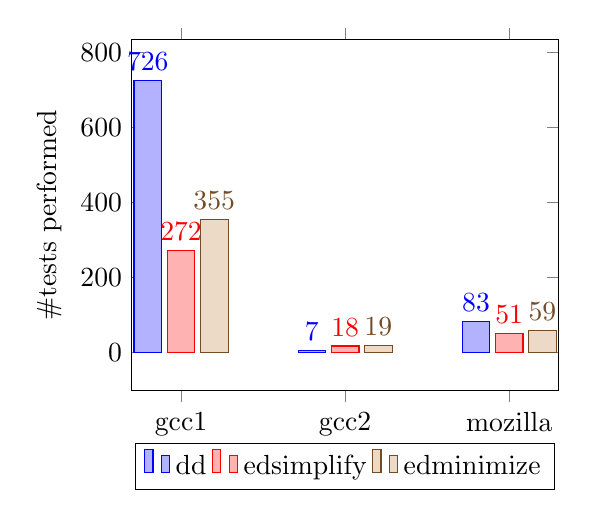
\begin{tikzpicture}
\begin{axis}[
    ybar,
    enlargelimits=0.15,
    legend style={at={(0.5,-0.15)},
      anchor=north,legend columns=-1},
    ylabel={\#tests performed},
    symbolic x coords={gcc1,gcc2,mozilla},
    xtick=data,
    nodes near coords,
    nodes near coords align={vertical},
    ]
\addplot coordinates {(gcc1,726) (gcc2,7) (mozilla,83)};
\addplot coordinates {(gcc1,272) (gcc2,18) (mozilla,51)};
\addplot coordinates {(gcc1,355) (gcc2,19) (mozilla,59)};
\legend{dd,edsimplify,edminimize}
\end{axis}
\end{tikzpicture}

As shown above, entropy debugging is able to minimize the first gcc crash input
in 52\% faster than delta debugging -- it is also able to simplify it in 37\% of
the time. Similarly, entropy debugging is 29\% faster at minimizing the mozilla
crash input, and can simplify it in 61\% of the time.

For the second gcc crash, entropy debugging takes nearly twice as long. Why?
The difference comes down to assumptions made by the algorithms. The input
contains 30 items, and the minimal subset is a single item. Delta Debugging
assumes this sort of input is likely, and the search it performs works out to be
a perfect binary search. On the other hand, Entropy Debugging assumes nothing
about the underlying information. It takes 10 checks just to presample the input
(with default hyperparameters), already losing to Delta Debugging. It then
executes 8 checks to simplify or 9 checks to minimize the input, which is
slightly behind Delta Debugging. In essence, the difference is the assumptions
made by the algorithms, combined with the small size of the input.

It is possible, in circumstances like this, to run entropy debugging without any
presampling, and to seed a custom starting probability distribution. In this
case, the second gcc crash input can be simplified by entropy debugging in six
checks. In general, this is not necesary, as Entropy Debugging beats
Delta Debugging for a very large range of markov model probabilities.

\subsection{Generated Data}

To more directly measure the point at which Delta Debugging may perform better,
than Entropy Debugging, generated data from various markov models are fed into
both algorithms and compared below. In addition, a naive brute force is plotted.
Delta Debugging often exceeds the naive approach by nearly 3x, while Entropy
Debugging fits itself to the curve.

\begin{figure}
  \centerline{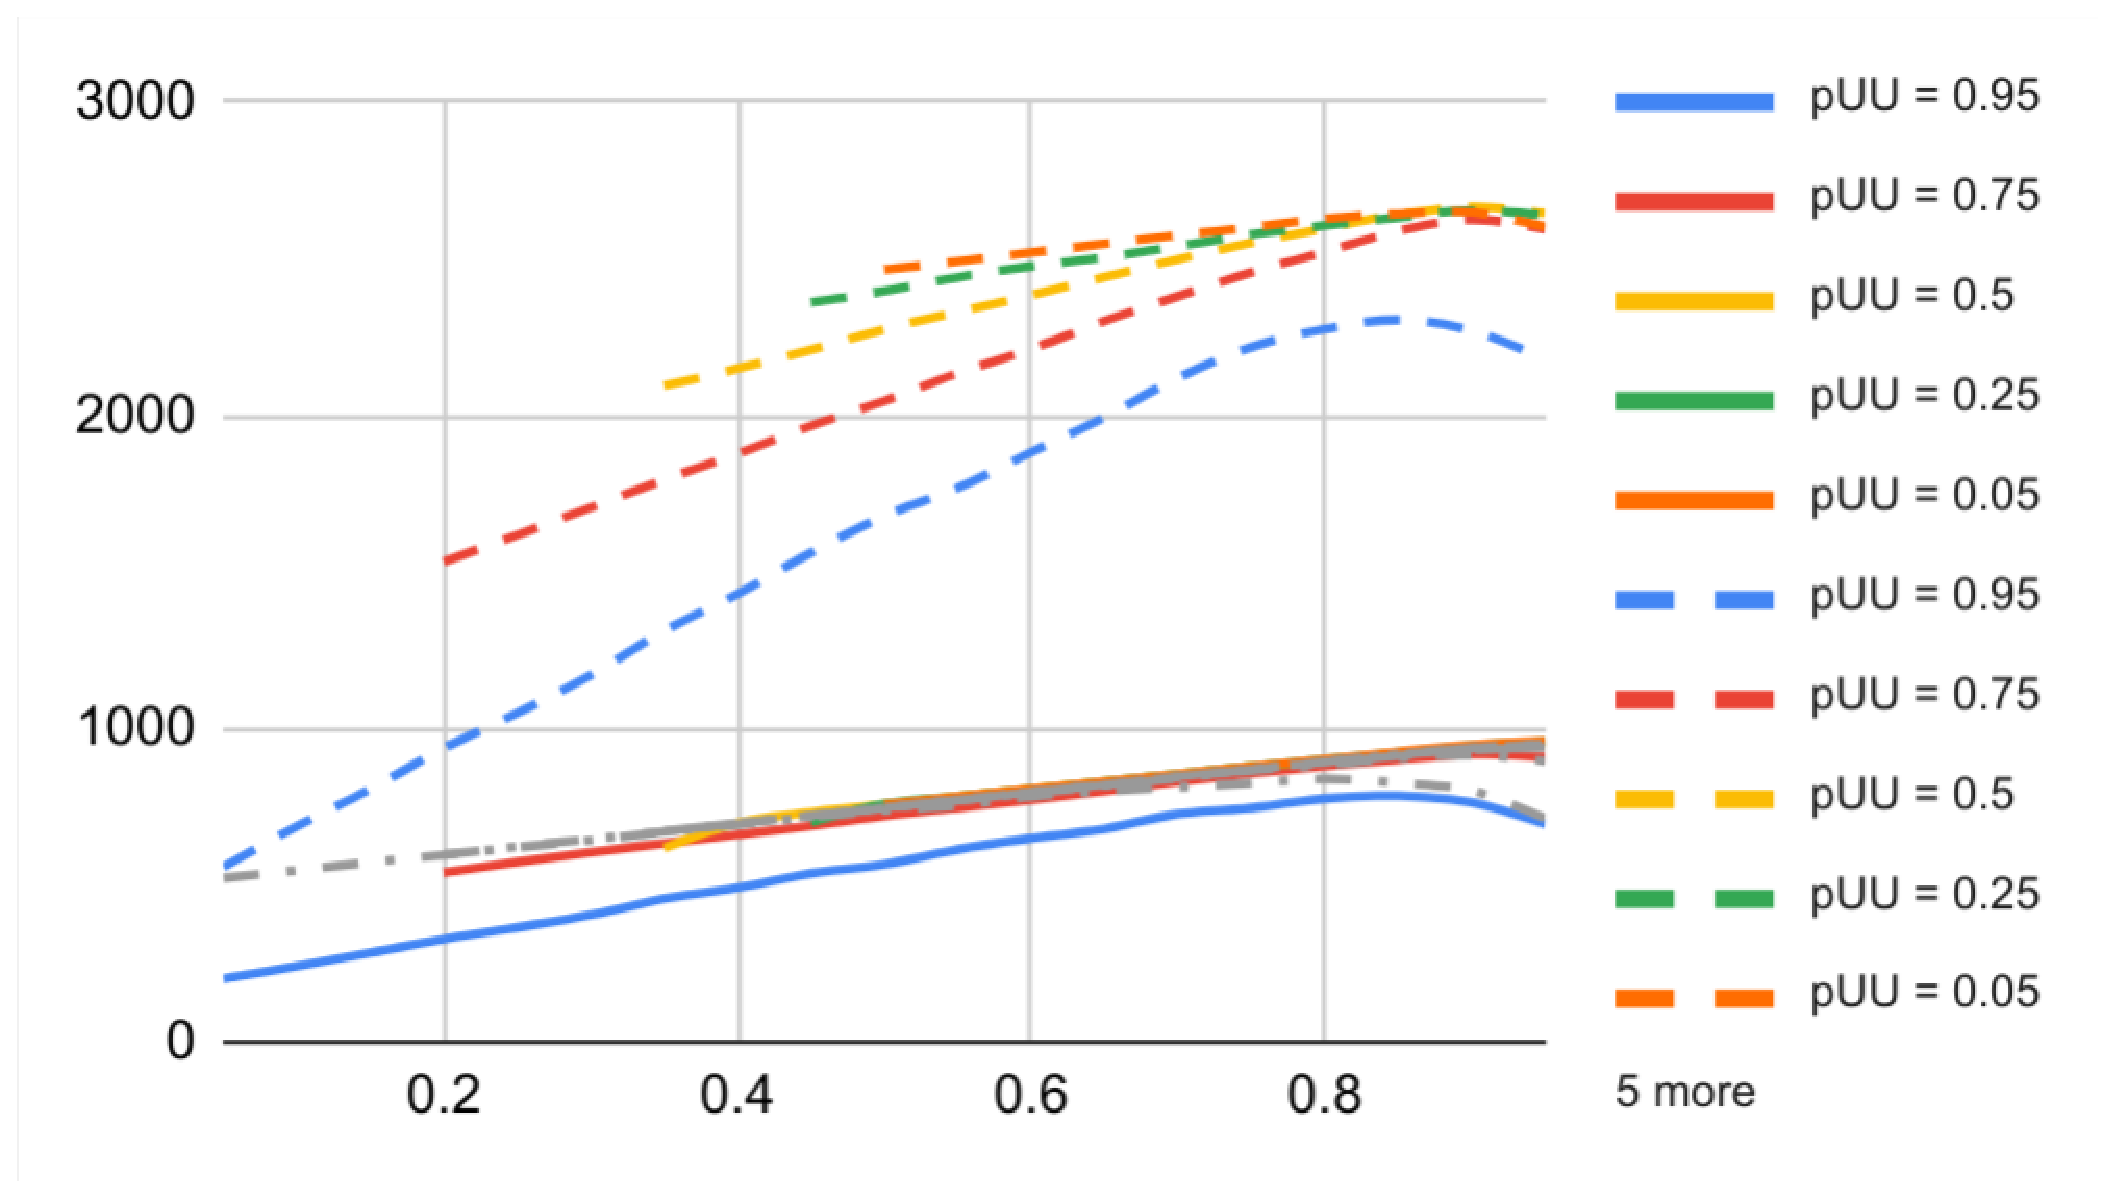
\includegraphics[scale=0.22]{generated_medium}}
  \caption{Delta debugging (dashed) vs brute force (grey), Entropy Debugging (solid) for medium probabilities}
%%\label{fig_example1.ps}
\end{figure}

In the above chart, Entropy Debugging is compared to Delta Debugging and a naive
brute force algorithm for "normal" markov probabilities. The x axis represents
the overall percentage of waste in an input, and the style of the line marks the
algorithm in question (solid = entropy debugging, dashed = Delta Debugging, grey
dash dot = brute force). Each algorithm is plotted for multiple transition
properties (correlation between waste/non-waste in the input): 95\% correlation,
75\% correlation, no correlation (50\%), 75\% discorrelation, 95\%
discorrelation.

For this range of probabilities, Delta Debugging only manages to approach the
performance of the naive solution in the most extreme case of 95\% waste with
95\% correlation. Indeed, Entropy Debugging is only considerably better than the
naive approach in the 95\% correlation plot (and never considerably worse).

This chart clearly does not capture a set of inputs that Delta Debugging was
designed to handle. As probabilities get further and further from these "normal"
(by some definition) probabilities, Delta Debugging gets closer and closer to
Entropy Debugging, with the two meeting when around 99.8\% of an input is waste
with around 99.9\% correlation.

\begin{figure}
  \centerline{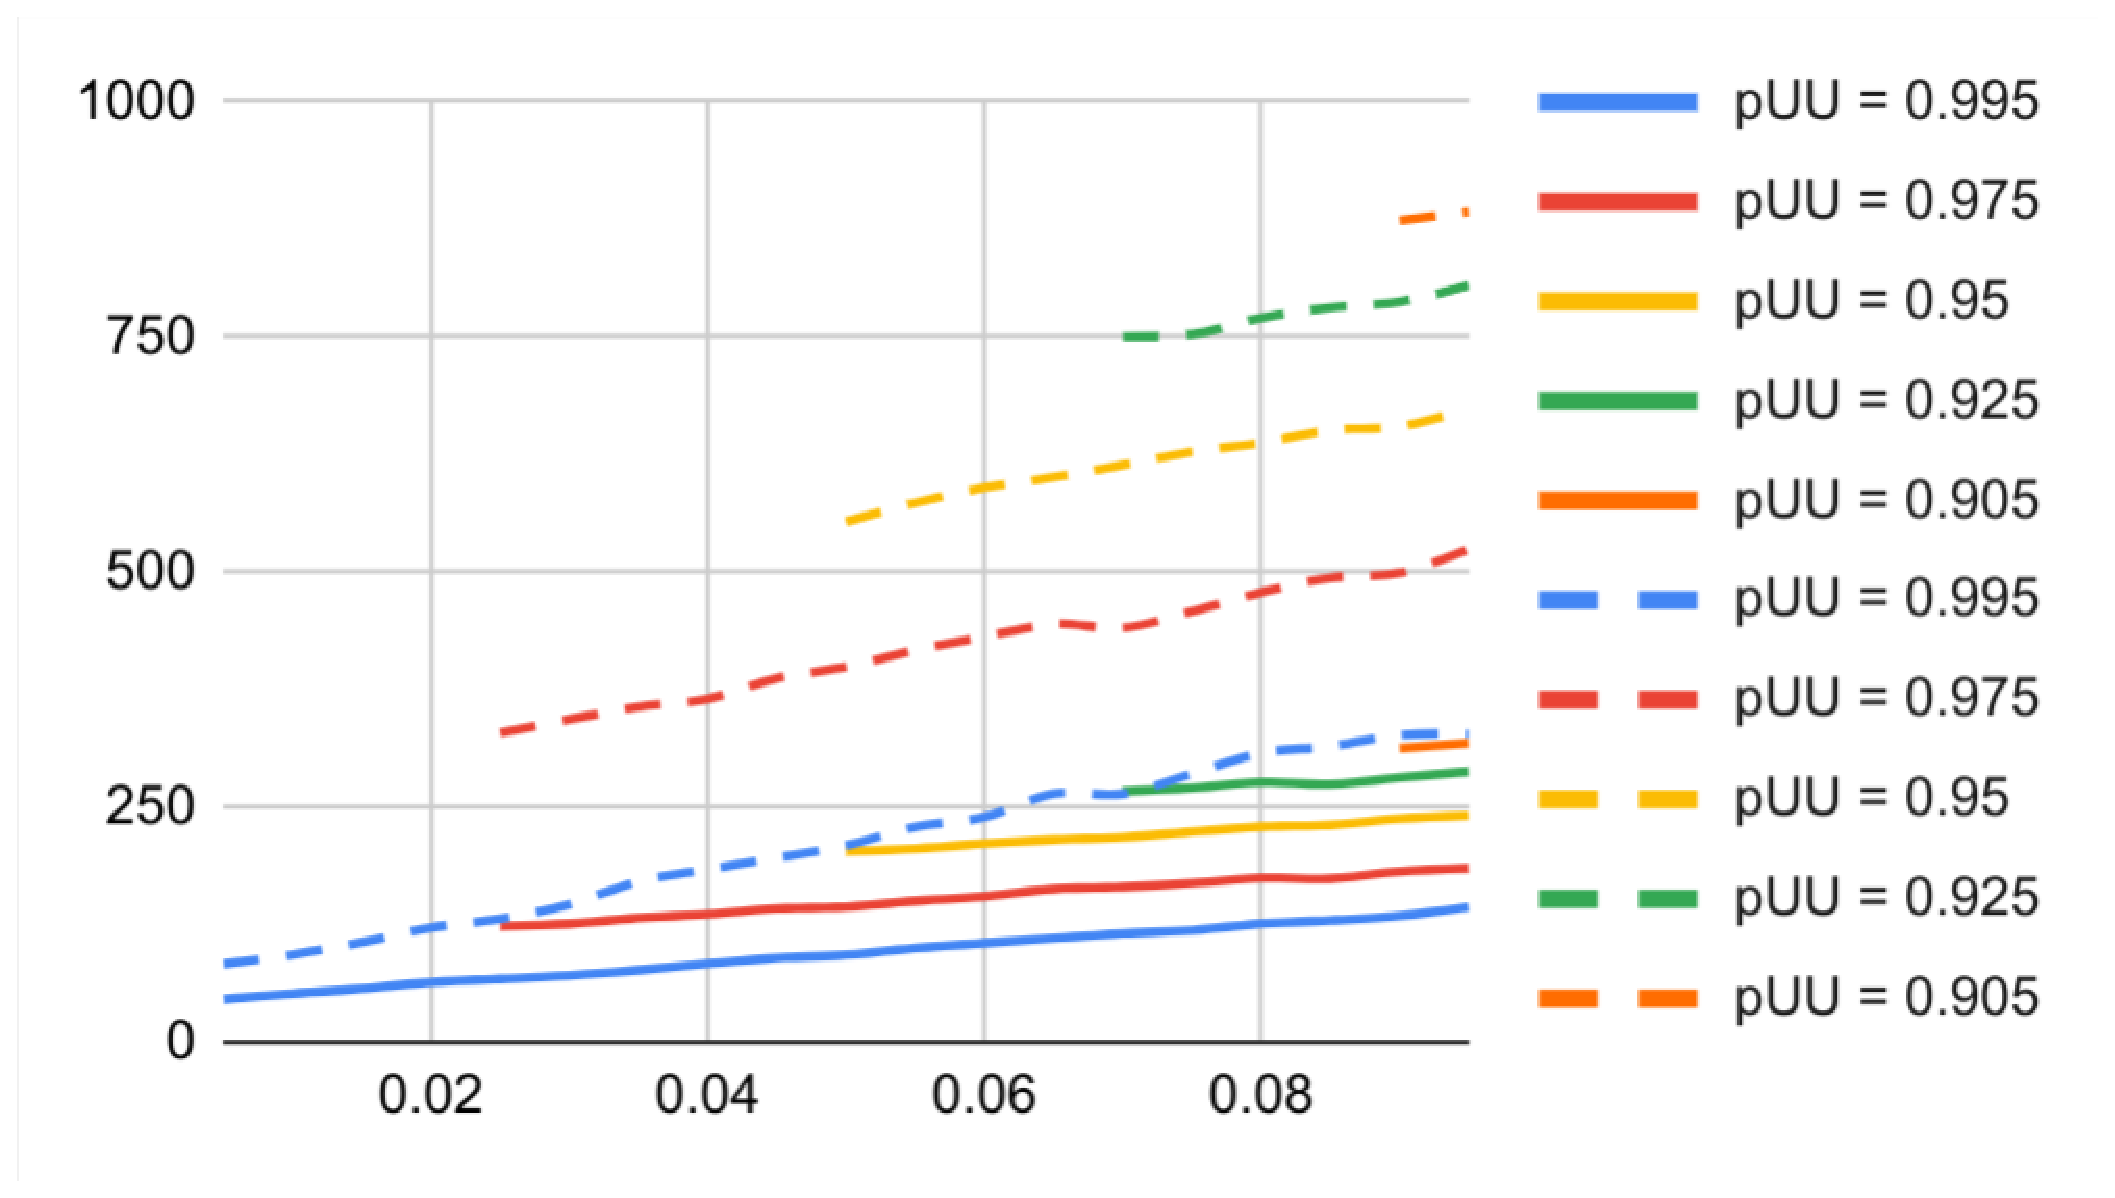
\includegraphics[scale=0.22]{generated_small}}
  \caption{Delta debugging (dashed) vs Entropy Debugging (solid) for small probabilities}
%%\label{fig_example1.ps}
\end{figure}

\begin{figure}
  \centerline{\includegraphics[scale=0.22]{generated_smallest}}
  \caption{Delta debugging (dashed) vs Entropy Debugging (solid) for very small probabilities}
%%\label{fig_example1.ps}
\end{figure}

\subsection{Fuzz Testing Coverage Corpus}

Entropy Debugging was used to minify a fuzz testing corpus while maintaining the
same code coverage.

The fuzzing library Dust is a code coverage guided fuzz testing framework for
Dart. This has been used to generate random Dart programs that may crash the
Dart analyzer. To do so, a corpus of interesting programs is maintained such
that those interesting programs each exercise some unique code path of the fuzz
target.

For the Dart language, there are hundreds of test files that cover most of the
language specification. This is therefore an ideal starting place to find this
set of interesting Dart programs. However, the corpus contains a lot of
redundancy from the perspective of any given fuzz target. The goal is to
therefore quickly minimize this corpus, a task that in theory should be a good
fit for either Delta Debugging or Entropy Debugging.

Here are four example simplifications, charted by input size to runs required by
the two algorithms. In the case of entropy debugging, it has been split out by
time required to simplify vs minimize the input.

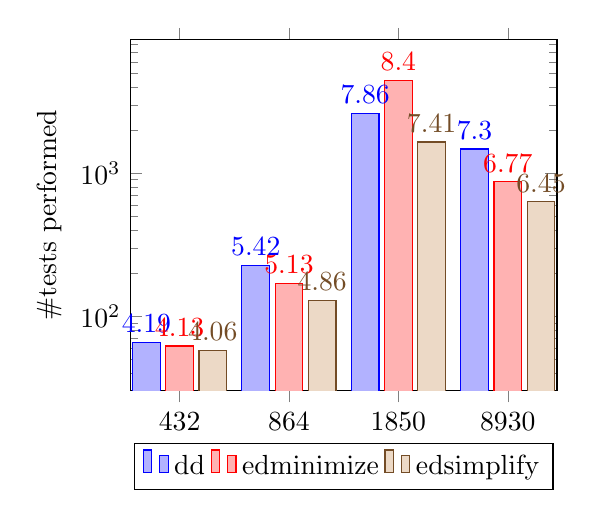
\begin{tikzpicture}
\begin{axis}[
    ybar,
    enlargelimits=0.15,
    legend style={at={(0.5,-0.15)},
      anchor=north,legend columns=-1},
    ylabel={\#tests performed},
    symbolic x coords={432,864,1850,8930},
    xtick=data,
    ymode=log,
    nodes near coords,
    nodes near coords align={vertical},
    ]
\addplot coordinates {(432,66) (864,227) (1850,2603) (8930,1476)};
\addplot coordinates {(432,62) (864,169) (1850,4463) (8930,869)};
\addplot coordinates {(432,58) (864,129) (1850,1653) (8930,630)};
\legend{dd,edminimize,edsimplify}
\end{axis}
\end{tikzpicture}

And here are the median, average, worst results of the three algorithms over
all samples.

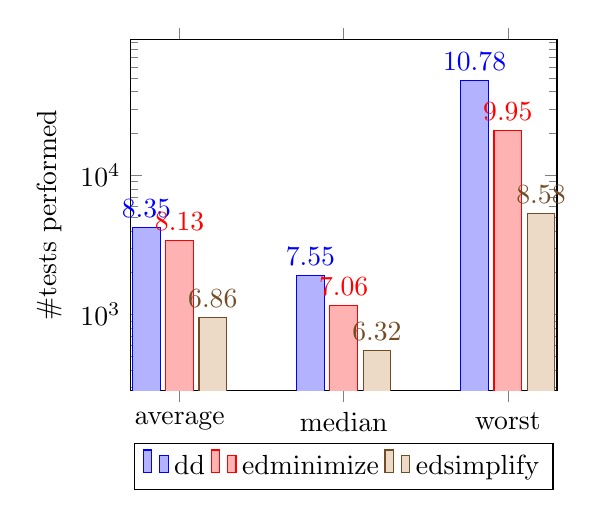
\begin{tikzpicture}
\begin{axis}[
    ybar,
    enlargelimits=0.15,
    legend style={at={(0.5,-0.15)},
      anchor=north,legend columns=-1},
    ylabel={\#tests performed},
    symbolic x coords={average,median,worst},
    xtick=data,
    ymode=log,
    nodes near coords,
    nodes near coords align={vertical},
    ]
\addplot coordinates {(median,1904) (average,4216) (worst,48156)};
\addplot coordinates {(median,1167) (average,3403) (worst,21000)};
\addplot coordinates {(median,557) (average,953) (worst,5330)};
\legend{dd,edminimize,edsimplify}
\end{axis}
\end{tikzpicture}

These data not only show not that Delta Debugging takes 80\% of the time in this
example in the average case, but it also took 43\% of the time in the worst
case.

\subsection{Is miminization useful?}

The previous numbers also raise the question of whether or not
\textit{minimization} is better than \textit{simplification}.

On average, minimization yielded an 11\% smaller input than simplification, even
though it took 3.5x as many tests. For context, the 11\% difference in the
result is a mere 3\% of the input -- and requires 33 additional tests per
additional removed character.

Of course, minimization is still posible with Entropy Debugging, and still
faster in this data set than Delta Debugging (especially in the median and worst
case). However, this paper finds no way to speed up minimization. Under the
statistical and compression theory approach described above, there simply is no
better approach than a character by character search when the entropy of a
sample is high. And at 89\% of the way simplified, that counts as high entropy.
And if a pass at this entropy ends up finding any items in the set that can be
removed, a new pass is required, creating pathological cases in both entropy
debugging as well as delta debugging.

Why is the average only 20\% less for Entropy Debugging even though its median
performance is a 40\% improvemnet from Delta Debugging, which also has the
highest worst case result? This is not a quantitative explanation, but it seems
the answer here is that an inefficient simplification stage leads to a better
minimization stage.

Recall that minimization in this paper specifically refers to Zeller's
definition of 1-minimal\cite{dd}. Stricter minimums can be sought such as
2-minimal and beyond. Anecdotally, it seems that acheiving 1-minimal may
frequently require removing \textit{pairs} or larger chunks of the input, more
in the realm of 2-minimal and beyond. In a character by character sweep, it may
take $n$ passes for some $n$ to acheive 1-minimality.

On the other hand, it seems that Delta Debugging is more likely to have run
additional suboptimal tests in the form of attempting to delete optimistically
large chunks of contiguous characters. These ultimately still result in a
larger average case performance, but they do decrease the likelihood of the
minimization stage taking a large number of passes. (Note that this effect also
does not keep Delta Debugging from claiming the largest recorded worst case
result).

It seems compelling that simplification is a good approximation of 1-minimal
that can be found in significantly less time. Future research to improve
minimization techniques seems prodent, and it seems likely that Delta Debugging
could also benefit from a simplification mode in addition to 1-minimal search.

Similarly, the case studies on mozilla and gcc could be even more drastically
improved if only a \textit{simplified} reproduction were sought instead of a
\textit{minmiized} one.

\subsection{Performance takeaways}

The benchmarking performed lends itself to a selection process between Entropy
Debugging and Delta Debugging.

If a true 1-minimal result is needed, it is possible that entropy-debugging will
not lead to significantly improved results without some improvement over the
process of minimization. However, it still appears to be the better algorithm in
the average and worst case.

If the input is likely close to simplified, Entropy Debugging will yield very
large improvements in performance over Delta Debugging.

If the input is small (approaching ~30 entries) and also far from the minimal
result, Delta Debugging may yield better results due to Entropy Debugging's
limitation of presampling (though this can be tuned).

If the input is very very far from the minimal result (less than 1\% of the
input, is expected to be part of the minimal result), then Delta Debugging may
yield better results due to Delta Debugging's more aggressive approach. This
may also be tunable as a hyperparameter of Entropy Debugging.

This paper proposes that in all other cases, Entropy Debugging seems to
outperform Delta Debugging in all other cases.

This paper also proposes that if a true \textit{minimal} result is \textit{not}
needed, that a simplification from the Entropy Debugging is a much more
efficient approximation.

\subsection{Optimality analysis}

To do: analyze how close entropy debugging gets to the lower bound of
algorithmic performance.

\subsection{Future Work}

There is a large body of future work to be explored in addition to this paper's
findings.

Entropy Debugging currently uses markov models as the only statistical
understanding of the simplification stream's information. This limits the
peformance of Entropy Debugging on inputs that could be described better by
better statistical models, such as machine learning models. While more advanced
models generally require more data, and data collection is itself throttled in
Entropy Debugging, it is possible that new statistical models could lead to
performance improvements, especially in simplifying large corpora of inputs.

Approaches to unify Entropy Debugging with hierarchical approaches such as
HDD\cite{hdd} could yield even larger efficiency. One possibility of such a
unification is to integrate the hierarchical nature of data into the statistical
models of Entropy Debugging rather than changing the overall structure of the
algorithm itself.

Delta Debugging is also capable of comparing minimum failing inputs with maximum
succeeding inputs. While Yu et. al. found that these isolated changes are
typically failure-irrelevant in practical usage\cite{ddRealPerspectives}, work
could be done to find these inputs as part of Entropy Debugging as well for
applications where it may be useful.

An algorithm remains to be found that can efficiently build an optimal runnable
identity encoding, or in general, an optimal ordered probabilistic tree. Doing
so may have implications for Decision Tree Learning in general, and would also
improve the performance of Entropy Debugging.

More advanced compression techniques than huffman code exists. Indeed, it is the
simplicity of huffman codes that make them easily applicable to this particular
simplification problem. However, it is possible that these more advanced
compression techniques such as Arithmetic Coding and ANS could be adapted to
produce runnable identity codes that could be used by Entropy Debugging.


%%%
%%%In order to get started in generating a two-column version of your paper, please format the document with 0.75in top margin, 1.5in bottom margin and 0.825in left and right margins.  Break the text into two sections one for the title heading, and another for the body of the paper.  
%%%
%%%The format of the heading is not critical, on the other hand formatting of the body of the text is the primary goal of this exercise.  This will allow you to see that the figures are matched to the column width and font size of the paper.  The double column of the heading section is set to 1.85in for the first column, a 0.5in spacing, and 4.5in for the second column.  For the body of the paper, set it to 3.34in for both columns with 0.17in spacing, both are right justified. 
%%%
%%%The information that is the focus of this exercise is found in 
%%%section~\ref{sect_figure}.
%%%Please use this template to format your paper in a way that is similar to the printed form of the Journal of Mechanical Design.  This will allow you to verify that the size and resolution of your figures match the page layout of the journal.  The ASME Journal of Mechanical Design will no longer publish papers that have the errors demonstrated here.
%%%
%%%ASME simply requires that the font should be the appropriate size and not be blurred or pixilated, and that lines should be the appropriate weight and have minimal, preferably no, pixilation or rasterization.
%%%
%%%The journal uses 10pt Times Roman Bold for headings, but Times Bold is good enough for this effort.  The text is set at 9pt Times Roman, and again Times will be fine.  Insert a new line after the heading, and two lines after each section.  This is not exactly right but it is close enough.
%%%
%%%
%%%%%%%%%%%%%%%%%%%%%%%%%%%%%%%%%%%%%%%%%%%%%%%%%%%%%%%%%%%%%%%%%%%%%%%%%
%%%\section{Very Very Very Very Very Very Very Very Very Very Very Long Heading}
%%%
%%%The heading is boldface with upper and lower case letters. 
%%%If the heading should run into more than one line, the run-over is not left-flushed.
%%%
%%%%%%%%%%%%%%%%%%%%%%%%%%%%%%%%%%%%%%%%%%%%%%%%%%%%%%%%%%%%%%%%%%%%%%%%%
%%%\subsection{Second-Level Heading}
%%%
%%%The next level of heading is also boldface with upper and lower case letters. 
%%%The heading is flushed left with the left margin. The spacing to the next heading is two line spaces.
%%%
%%%%%%%%%%%%%%%%%%%%%%%%%%%%%%%%%%%%%%%%%%%%%%%%%%%%%%%%%%%%%%%%%%%%%%%%%
%%%\subsubsection{Third-Level Heading.}
%%%
%%%The third-level of heading follows the style of the second-level heading.
%%%
%%%
%%%%%%%%%%%%%%%%%%%%%%%%%%%%%%%%%%%%%%%%%%%%%%%%%%%%%%%%%%%%%%%%%%%%%%%%%
%%%\section{Use of SI Units}
%%%
%%%An ASME paper should use SI units.  When preference is given to SI units, the U.S. customary units may be given in parentheses or omitted. When U.S. customary units are given preference, the SI equivalent {\em shall} be provided in parentheses or in a supplementary table. 
%%%
%%%%%%%%%%%%%%%%%%%%%%%%%%%%%%%%%%%%%%%%%%%%%%%%%%%%%%%%%%%%%%%%%%%%%%%%%
%%%\section{Footnotes\protect\footnotemark}
%%%\footnotetext{Examine the input file, asme2ej.tex, to see how a footnote is given in a head.}
%%%
%%%Footnotes are referenced with superscript numerals and are numbered consecutively from 1 to the end of the paper\footnote{Avoid footnotes if at all possible.}. Footnotes should appear at the bottom of the column in which they are referenced.
%%%
%%%
%%%%%%%%%%%%%%%%%%%%%%%%%%%%%%%%%%%%%%%%%%%%%%%%%%%%%%%%%%%%%%%%%%%%%%%%%
%%%\section{Mathematics}
%%%
%%%Equations should be numbered consecutively beginning with (1) to the end of the paper, including any appendices.  The number should be enclosed in parentheses and set flush right in the column on the same line as the equation.  An extra line of space should be left above and below a displayed equation or formula. \LaTeX\ can automatically keep track of equation numbers in the paper and format almost any equation imaginable. An example is shown in Eqn.~(\ref{eq_ASME}). The number of a referenced equation in the text should be preceded by Eqn.\ unless the reference starts a sentence in which case Eqn.\ should be expanded to Equation.
%%%
%%%\begin{equation}
%%%f(t) = \int_{0_+}^t F(t) dt + \frac{d g(t)}{d t}
%%%\label{eq_ASME}
%%%\end{equation}
%%%
%%%%%%%%%%%%%%%%%%%%%%%%%%%%%%%%%%%%%%%%%%%%%%%%%%%%%%%%%%%%%%%%%%%%%%%%%
%%%\section{Figures}
%%%\label{sect_figure}
%%%
%%%All figures should be positioned at the top of the page where possible.  All figures should be numbered consecutively and centered under the figure as shown in Fig.~\ref{figure_ASME}. All text within the figure should be no smaller than 7~pt. There should be a minimum two line spaces between figures and text. The number of a referenced figure or table in the text should be preceded by Fig.\ or Tab.\ respectively unless the reference starts a sentence in which case Fig.\ or Tab.\ should be expanded to Figure or Table.
%%%
%%%
%%%%%%%%%%%%%%%%%%%%%%%%%%%%%%%%%%%%%%%%%%%%%%%%%%%%%%%%%%%%%%%%%%%%%%%%%
%%%%%%%%%%%%%%%%%%% begin figure %%%%%%%%%%%%%%%%%%%
%%%\begin{figure}[t]
%%%\begin{center}
%%%\setlength{\unitlength}{0.012500in}%
%%%\begin{picture}(115,35)(255,545)
%%%\thicklines
%%%\put(255,545){\framebox(115,35){}}
%%%\put(275,560){Beautiful Figure}
%%%\end{picture}
%%%\end{center}
%%%\caption{The caption of a single sentence does not have period at the end}
%%%\label{figure_ASME} 
%%%\end{figure}
%%%%%%%%%%%%%%%%%%% end figure %%%%%%%%%%%%%%%%%%% 
%%%%%%%%%%%%%%%%%%%%%%%%%%%%%%%%%%%%%%%%%%%%%%%%%%%%%%%%%%%%%%%%%%%%%%%%%
%%%
%%%In the following subsections, I have inserted figures that have been provided by authors in order to demonstrate what to avoid.  In each case the authors provided figures that are 3.25in wide and 600dpi in the .tif graphics format.  The papers containing these figures have been held from production due to their poor quality. 
%%%
%%%%%%%%%%%%%%%%%%%%%%%%%%%%%%%%%%%%%%%%%%%%%%%%%%%%%%%%%%%%%%%%%%%%%%%%%
%%%\subsection{The 1st Example of Bad Figure}
%%%
%%%%%%%%%%%%%%%%%%% begin figure %%%%%%%%%%%%%%%%%%%
%%%%%% 3.34in is the maximum width you can have for a figure
%%%\begin{figure} 
%%%\centerline{\psfig{figure=figure/FMANU_MD_05_1107_11.ps,width=3.34in}}
%%%\caption{Example taken from a paper that was held from production because the image quality is poor.  ASME sets figures captions in 8pt, Helvetica Bold.}
%%%\label{fig_example1.ps}
%%%\end{figure}
%%%%%%%%%%%%%%%%%%% end figure %%%%%%%%%%%%%%%%%%%
%%%
%%%In order to place the figure in this template using MSWord, select ����Insert Picture from File,���� and use wrapping that is  ����top and bottom.����  Make sure the figure is 3.25in wide.
%%% 
%%%Figure~`\ref{fig_example1.ps}
%%%was taken from a recent paper that was held from publication, because the text is fuzzy and unreadable.  It was probably obtained by taking a screen shot of the computer output of the author����s software.  This means the original figure was 72dpi (dots per inch) on a computer screen.  There is no way to improve the quality such a low resolution figure.
%%% 
%%%In order to understand how poor the quality of this figure is, please zoom in slightly, say to 200\%.  Notice that while the font of the paper is clear at this size, the font in the figures is fuzzy and blurred.  It is impossible to make out the small symbol beside the numbers along the abscissa of the graph.  Now consider the labels ����Time���� and ����Cost.����  They are clearly in fonts larger that the text of the article, yet the pixilation or rasterization, associated with low resolution is obvious. This figure must be regenerated at higher resolution to ensure quality presentation.
%%%
%%%The poor quality of this figure is immediately obvious on the printed page, and reduces the impact of the research contribution of the paper, and in fact detracts from the perceived quality of the journal itself.
%%%
%%%
%%%
%%%%%%%%%%%%%%%%%%%%%%%%%%%%%%%%%%%%%%%%%%%%%%%%%%%%%%%%%%%%%%%%%%%%%%%%%
%%%\subsection{The 2nd Example of Bad Figure}
%%%
%%%%%%%%%%%%%%%%%%% begin figure %%%%%%%%%%%%%%%%%%%
%%%\begin{figure} 
%%%\centerline{\psfig{figure=figure/FMANU_MD_05_1272_5.ps,width=3.34in}}
%%%\caption{While this figures is easily readable at a double column width of 6.5in, when it is shrunk to 3.25in column width the text is unreadable.   This paper was held from production.}
%%%\label{fig_example2.ps}
%%%\end{figure}
%%%%%%%%%%%%%%%%%%% end figure %%%%%%%%%%%%%%%%%%%
%%%
%%%Figure~\ref{fig_example2.ps}
%%%demonstrates a common problem that arises when a figure is scaled down fit a single column width of 3.25in.  The original figure had labels that were readable at full size, but become unreadable when scaled to half size.  This figure also suffers from poor resolution as is seen in the jagged lines the ovals that form the chain.
%%%
%%%This problem can be addressed by increasing the size of the figure to a double column width of 6.5in, so the text is readable.  But this will not improve the line pixilation, and a large low resolution figure is less desirable than a small one.  This also significantly expands the length of the paper, and may cause it to exceed the JMD nine page limit.  Additional pages require page charges of \$200 per page.  It is best to regenerate the figure at the resolution that ensures a quality presentation.
%%%
%%%
%%%%%%%%%%%%%%%%%%%%%%%%%%%%%%%%%%%%%%%%%%%%%%%%%%%%%%%%%%%%%%%%%%%%%%%%%
%%%\subsection{The 3rd Example of Bad Figure}
%%%%%%%%%%%%%%%%%%% begin figure %%%%%%%%%%%%%%%%%%%
%%%\begin{figure} 
%%%%\centerline{\psfig{figure=figure/FMANU_MD_04_1274_13.ps,width=3.34in}}
%%%\centerline{\psfig{figure=figure/FMANU_MD_04_1274_13.ps,width=3.25in}}
%%%\caption{Another example of a figure with unreadable text.  Even when the paper was expanded to double column width the text as shown in Fig.~\ref{fig_example4.ps} was of such low quality that the paper was held from production.}
%%%\label{fig_example3.ps}
%%%\end{figure}
%%%%%%%%%%%%%%%%%%% end figure %%%%%%%%%%%%%%%%%%%
%%%
%%%%%%%%%%%%%%%%%%% begin figure %%%%%%%%%%%%%%%%%%%
%%%%%% the maximum width in double column is 6.85in
%%%\begin{figure*} 
%%%\centerline{\psfig{figure=figure/FMANU_MD_04_1274_13.ps,width=6.85in}}
%%%\caption{A figure expanded to double column width the text from Figure~\ref{fig_example3.ps}}
%%%\label{fig_example4.ps}
%%%\end{figure*}
%%%%%%%%%%%%%%%%%%% end figure %%%%%%%%%%%%%%%%%%%
%%%An author provided the high resolution image 
%%%in Fig.~\ref{fig_example3.ps}
%%%that was sized to a single column width of 3.25in.  Upon seeing the poor quality of the text, the publisher scaled the image to double column width as shown in Fig.~\ref{fig_example4.ps} 
%%%at which point it took half of a page.  The publisher went on to do this for all eight figures generating four pages of figures that the author did not expect. ASME stopped production of the paper even with the larger figures due to the pixilation of the font.
%%%
%%%Clearly the text in this figure is unreadable, and it is doubtful that the author can print the output in a way that it is readable.  This is a problem that the author must solve, not the publisher. 
%%%
%%%As you might expect, I have many more examples, but in the end the author is the best judge of what is needed in each figure.  ASME simply requires that the image meet a minimum standard for font and line quality, specifically the font should be the appropriate size and not be blurred or pixilated, and that lines should be the appropriate weight and have minimal, preferably no, pixilation or rasterization.
%%%
%%%
%%%%%%%%%%%%%%%%%%%%%%%%%%%%%%%%%%%%%%%%%%%%%%%%%%%%%%%%%%%%%%%%%%%%%%%%%
%%%\section{Tables}
%%%
%%%%%%%%%%%%%%%%%%%%%%%%%%%%%%%%%%%%%%%%%%%%%%%%%%%%%%%%%%%%%%%%%%%%%%%%%
%%%%%%%%%%%%%%%%%% begin table   %%%%%%%%%%%%%%%%%%%%%%%%%%
%%%\begin{table}[t]
%%%\caption{Figure and table captions do not end with a period}
%%%\begin{center}
%%%\label{table_ASME}
%%%\begin{tabular}{c l l}
%%%& & \\ % put some space after the caption
%%%\hline
%%%Example & Time & Cost \\
%%%\hline
%%%1 & 12.5 & \$1,000 \\
%%%2 & 24 & \$2,000 \\
%%%\hline
%%%\end{tabular}
%%%\end{center}
%%%\end{table}
%%%%%%%%%%%%%%%%%%% end table %%%%%%%%%%%%%%%%%%% 
%%%%%%%%%%%%%%%%%%%%%%%%%%%%%%%%%%%%%%%%%%%%%%%%%%%%%%%%%%%%%%%%%%%%%%%%%
%%%
%%%All tables should be numbered consecutively  and centered above the table as shown in Table~\ref{table_ASME}. The body of the table should be no smaller than 7 pt.  There should be a minimum two line spaces between tables and text.
%%%
%%%
%%%%%%%%%%%%%%%%%%%%%%%%%%%%%%%%%%%%%%%%%%%%%%%%%%%%%%%%%%%%%%%%%%%%%%%%%
%%%\section{Citing References}
%%%
%%%%%%%%%%%%%%%%%%%%%%%%%%%%%%%%%%%%%%%%%%%%%%%%%%%%%%%%%%%%%%%%%%%%%%%%%
%%%The ASME reference format is defined in the authors kit provided by the ASME.  The format is:
%%%
%%%\begin{quotation}
%%%{\em Text Citation}. Within the text, references should be cited in  numerical order according to their order of appearance.  The numbered reference citation should be enclosed in brackets.
%%%\end{quotation}
%%%
%%%The references must appear in the paper in the order that they were cited.  In addition, multiple citations (3 or more in the same brackets) must appear as a `` [1-3]''.  A complete definition of the ASME reference format can be found in the  ASME manual \cite{asmemanual}.
%%%
%%%The bibliography style required by the ASME is unsorted with entries appearing in the order in which the citations appear. If that were the only specification, the standard {\sc Bib}\TeX\ unsrt bibliography style could be used. Unfortunately, the bibliography style required by the ASME has additional requirements (last name followed by first name, periodical volume in boldface, periodical number inside parentheses, etc.) that are not part of the unsrt style. Therefore, to get ASME bibliography formatting, you must use the \verb+asmems4.bst+ bibliography style file with {\sc Bib}\TeX. This file is not part of the standard BibTeX distribution so you'll need to place the file someplace where LaTeX can find it (one possibility is in the same location as the file being typeset).
%%%
%%%With \LaTeX/{\sc Bib}\TeX, \LaTeX\ uses the citation format set by the class file and writes the citation information into the .aux file associated with the \LaTeX\ source. {\sc Bib}\TeX\ reads the .aux file and matches the citations to the entries in the bibliographic data base file specified in the \LaTeX\ source file by the \verb+\bibliography+ command. {\sc Bib}\TeX\ then writes the bibliography in accordance with the rules in the bibliography .bst style file to a .bbl file which \LaTeX\ merges with the source text.  A good description of the use of {\sc Bib}\TeX\ can be found in \cite{latex, goosens} (see how two references are handled?).  The following is an example of how three or more references \cite{latex, asmemanual,  goosens} show up using the \verb+asmems4.bst+ bibliography style file in conjunction with the \verb+asme2ej.cls+ class file. Here are some more \cite{art, blt, ibk, icn, ips, mts, mis, pro, pts, trt, upd} which can be used to describe almost any sort of reference.
%%%
%%%%%%%%%%%%%%%%%%%%%%%%%%%%%%%%%%%%%%%%%%%%%%%%%%%%%%%%%%%%%%%%%%%%%%%%%
\section{Conclusions}
Conclusions TBD
%%%
%%%This gives you the opportunity to ensure that the figures are sized appropriately, in particular that the labels are readable and match the size of the text in the journal, and that the line weights and resolutions have no pixilation or rasterization.  Poor quality figures are immediately obvious on the printed page, and this detracts from the perceived quality of the journal.
%%%
%%%I am pleased to provide advice on how to improve any figure, but this effort must start with a two-column version of the manuscript. Thank you in advance for your patience with this effort, it will ensure quality presentation of your research contributions.
%%%
%%%
%%%
%%%%%%%%%%%%%%%%%%%%%%%%%%%%%%%%%%%%%%%%%%%%%%%%%%%%%%%%%%%%%%%%%%%%%%%%%
\section{Discussions}
Discussion TBD
%%%More specifically, the following features are not ASME format compliant.
%%%\begin{enumerate}
%%%\item
%%%The format for the title, author, and abstract in the cover page.
%%%\item
%%%The font for title should be 24 pt Helvetica bold.
%%%\end{enumerate}
%%%
%%%\noindent
%%%If you can help to fix these problems, please send us an updated template.
%%%If you know there is any other non-compliant item, please let us know.
%%%We will add it to the above list.
%%%With your help, we shall make this template 
%%%compliant to the ASME journal paper format.
%%%
%%%
%%%%%%%%%%%%%%%%%%%%%%%%%%%%%%%%%%%%%%%%%%%%%%%%%%%%%%%%%%%%%%%%%%%%%%%%%
\begin{acknowledgment}
Acknowledgement TBD
\end{acknowledgment}

%%%%%%%%%%%%%%%%%%%%%%%%%%%%%%%%%%%%%%%%%%%%%%%%%%%%%%%%%%%%%%%%%%%%%%
% The bibliography is stored in an external database file
% in the BibTeX format (file_name.bib).  The bibliography is
% created by the following command and it will appear in this
% position in the document. You may, of course, create your
% own bibliography by using thebibliography environment as in
%
% \begin{thebibliography}{12}
% ...
% \bibitem{itemreference} D. E. Knudsen.
% {\em 1966 World Bnus Almanac.}
% {Permafrost Press, Novosibirsk.}
% ...
% \end{thebibliography}

% Here's where you specify the bibliography style file.
% The full file name for the bibliography style file 
% used for an ASME paper is asmems4.bst.
\bibliographystyle{asmems4}

% Here's where you specify the bibliography database file.
% The full file name of the bibliography database for this
% article is asme2e.bib. The name for your database is up
% to you.
\bibliography{entropy-debugging}
%%%
%%%%%%%%%%%%%%%%%%%%%%%%%%%%%%%%%%%%%%%%%%%%%%%%%%%%%%%%%%%%%%%%%%%%%%%%%
%%%\appendix       %%% starting appendix
%%%\section*{Appendix A: Head of First Appendix}
%%%Avoid Appendices if possible.
%%%
%%%%%%%%%%%%%%%%%%%%%%%%%%%%%%%%%%%%%%%%%%%%%%%%%%%%%%%%%%%%%%%%%%%%%%%%%
%%%\section*{Appendix B: Head of Second Appendix}
%%%\subsection*{Subsection head in appendix}
%%%The equation counter is not reset in an appendix and the numbers will
%%%follow one continual sequence from the beginning of the article to the very end as shown in the following example.
%%%\begin{equation}
%%%a = b + c.
%%%\end{equation}

\end{document}
